\documentclass{article}
\usepackage[utf8]{inputenc}
\usepackage[T1]{fontenc}
\usepackage[portuguese]{babel}

\usepackage{indentfirst}
\usepackage{makeidx}
\usepackage{stackengine}
\usepackage{amssymb}
\usepackage{amsthm}
\usepackage{hyperref}
\usepackage{color}
\usepackage{graphicx}

\usepackage{pdfpages}
\usepackage{float}

\usepackage{booktabs}

\usepackage[showframe=false]{geometry}
\usepackage{changepage}


\title{\bf{Aprendizagem Computacional - Trabalho Prático 4}\vspace{80mm}}
\author{\textbf{João Tiago Márcia do Nascimento Fernandes - 2011162899} \\
\textbf{Joaquim Pedro Bento Gonçalves Pratas Leitão - 2011150072}}
\makeindex

\begin{document}

\maketitle

\pagebreak

\renewcommand*\contentsname{Índice}
\tableofcontents

\pagebreak

\section{Introdução}

O presente trabalho visa a implementação de controladores difusos de um dado sistema, dos tipos \emph{Mamdani} e \emph{Sugeno}, e que representam um hipotético processo real, tendo como base do seu funcionamento regras da \emph{lógica difusa}.

\vspace{.3cm}

A \emph{lógica difusa} extende o conceito de \emph{lógica booleana}, admitindo valores lógicos intermediários entre os valores de \emph{FALSO} e \emph{VERDADEIRO}. Assim, a lógica difusa permite-nos extender o conceito de conjunto, permitindo que um elemento passe a possuir um \emph{grau de pertença} num dado conjunto, cujo valor varia entre \emph{0} e \emph{1}.

\vspace{.3cm}

Relativamente aos controladores referidos, estes foram desenvolvidos no ambiente \emph{Simulink}, em conjunto com a \emph{Fuzzy Logic Toolbox}, ambos pertencentes à plataforma \emph{Matlab}. Numa fase inicial do trabalho apenas foram desenvolvidos controladores de \emph{9} regras, tendo posteriormente aumentado o seu número de regras para um total de \emph{25}.

\vspace{.3cm}

No presente documento pretendemos apresentar de forma mais detalhada os controladores implementados, discutindo alguns detalhes relativos à sua implementação e apresentando uma reflexão crítica sobre o desempenho e performance dos diferentes controladores implementados (\emph{Mamdani} e \emph{Sugeno}, de \emph{9} e \emph{25} regras).


\pagebreak

\section{Aplicação Desenvolvida}

A aplicação desenvolvida visa implementar os controladores difusos referidos anteriormente, representando um hipotético processo real, cujo funcionamento pode ser simulado, através da aplicação.

Para isso, a aplicação foi implementada em \emph{Matlab}, recorrendo à \emph{Fuzzy Logic Toolbox} do \emph{Simulink}, de forma a permitir a simulação do processo.

A aplicação faz ainda uso de uma interface por linha de comandos (\emph{CLI - Command Line Interface}), que permite ao utilizador escolher as características do processo que pretende simular: tipo de controlador, número de regras e tipos de perturbações, referência, entre outros.

\subsection{Referências}

Falar das duas referências disponibilizadas: Onda quadrada e Seno (Ambas com amplitude 1)

\subsection{Controladores}

Falar nos controladores implementados: Mamdani e Sugeno de 9 e 25 regras. Meter imagens com as regras, e explicar para que é que servem (ajustar/corrigir a saida de acordo com o erro actual e com a sua variaçao).

Falar também do ajuste das escalas que tivémos de fazer

\subsection{Perturbações}

Falar nas diferentes perturbações implementadas: Ausência de perturbação; Perturbação no actuador; Perturbação na carga; Perturbação no actuador e na carga

Tentar explicar alguma coisa sobre isto, eventualmente do que seria de esperar como resultado em cada uma das situações??

\subsection{Implementação}

Falar nos principais ficheiros que constituem a aplicação -- Meter isso numa secção chamada "Implementação no Simulink" - Meter imagem de uma das implementações

\subsubsection{Models}

Explicar que nesta pasta estão os modelos do sistema, dizer que foram implementados no simulink, e que são executados a partir dele

\subsection{Controllers}

Explicar que nesta pasta estão os controladores implementados, e que foram implementados no simulink, recorrendo ao fiseditor

\subsubsection{run.m}

Explicar como executar este ficheiro -- Ver readme.txt


\subsection{Execução}

Indicar como se deve executar a aplicação


\pagebreak

\section{Testes da Aplicação}

%Falar nos testes que realizámos e nos resultados que obtivémos (Fazer testes com e sem perturbador nos actuadores)

%Falar nos factores de escala utilizados: 1/10 antes do controlador e 10 depois do controlador

%Façam o estudo de desempenho do controlador em relação aos 3 objetivos:
%	1- seguir a referência
%	2- compensar a perturbação na carga
%	3- compensar a perturbação no atuador.

%Meter tabela com performance de cada teste
\begin{table}[h]
\begin{adjustwidth}{-1cm}{}
\begin{tabular}{|p{1.7cm}|p{2.55cm}|p{3cm}|p{2.5cm}|p{2.5cm}|p{2.2cm}|}
\hline
\textbf{Controller} & \textbf{Number Rules} & \textbf{Signal Generator} & \textbf{Perturbation Actuator} & \textbf{Perturbation Charge} & \textbf{Performance} \\ \hline
Mamdani             & 9                     & Square                    & No                             & No                           & 86.23                \\
Mamdani             & 9                     & Square                    & Yes                            & No                           & 98.55                \\
Mamdani             & 9                     & Square                    & No                             & Yes                          & 104.3                \\
Mamdani             & 9                     & Square                    & Yes                            & Yes                          & 116                  \\
Mamdani             & 9                     & Sin                       & No                             & No                           & 0.008748             \\
Mamdani             & 9                     & Sin                       & Yes                            & No                           & 10.4                 \\
Mamdani             & 9                     & Sin                       & No                             & Yes                          & 6.464                \\
Mamdani             & 9                     & Sin                       & Yes                            & Yes                          & 19.38                \\
Mamdani             & 25                    & Square                    & No                             & No                           & 25.67                \\
Mamdani             & 25                    & Square                    & Yes                            & No                           & 26.23                \\
Mamdani             & 25                    & Square                    & No                             & Yes                          & 27.14                \\
Mamdani             & 25                    & Square                    & Yes                            & Yes                          & 30.99                \\
Mamdani             & 25                    & Sin                       & No                             & No                           & 0.0002281            \\
Mamdani             & 25                    & Sin                       & Yes                            & No                           & 0.3861               \\
Mamdani             & 25                    & Sin                       & No                             & Yes                          & 1.425                \\
Mamdani             & 25                    & Sin                       & Yes                            & Yes                          & 2.865                \\
Sugeno              & 9                     & Square                    & No                             & No                           & 22                   \\
Sugeno              & 9                     & Square                    & Yes                            & No                           & 22.45                \\
Sugeno              & 9                     & Square                    & No                             & Yes                          & 26.11                \\
Sugeno              & 9                     & Square                    & Yes                            & Yes                          & 27.62                \\
Sugeno              & 9                     & Sin                       & No                             & No                           & 0.0002019            \\
Sugeno              & 9                     & Sin                       & Yes                            & No                           & 0.2998               \\
Sugeno              & 9                     & Sin                       & No                             & Yes                          & 1.495                \\
Sugeno              & 9                     & Sin                       & Yes                            & Yes                          & 2.689                \\
Sugeno              & 25                    & Square                    & No                             & No                           & 21.98                \\
Sugeno              & 25                    & Square                    & Yes                            & No                           & 22.77                \\
Sugeno              & 25                    & Square                    & No                             & Yes                          & 25.77                \\
Sugeno              & 25                    & Square                    & Yes                            & Yes                          & 27.49                \\
Sugeno              & 25                    & Sin                       & No                             & No                           & 0.0001569            \\
Sugeno              & 25                    & Sin                       & Yes                            & No                           & 0.2356               \\
Sugeno              & 25                    & Sin                       & No                             & Yes                          & 1.489                \\
Sugeno              & 25                    & Sin                       & Yes                            & Yes                          & 2.594\\ \hline               
\end{tabular}

\caption{Resultados dos Testes Realizados}
\end{adjustwidth}
\end{table}

\pagebreak

\section{Conclusões}

Reflexão sobre o trabalho e sobre os resultados obtidos - À partida será de esperar que os controladores com 25 regras apresentem melhores resultados que os controladores com apenas 9 regras --> Confirmar se isso se verificou e identificar qual o controlador (Mamdani ou Sugeno) que apresentou melhores resultados

Meter algumas imagens dos resultados dos testes: Salientar aqueles aspectos de quando o valor obtido é inferior ao esperado ele corrige aumentado, logo o vlor obtido vai subir, depois sobe demais e tem que descer, etc

\pagebreak

\section{Anexos}

Nesta secção apresentamos os resultados obtidos em cada teste realizado ao processo: Para além da performance registada (e que pode ser consultada na 3ª secção deste documento) registámos também a saída obtida e esperada para cada processo, a partir das quais foi calculada a sua performance.

\vspace{.2cm}

%======================Mamdani_9_square=====================================

\begin{figure}[h]
  \centering
      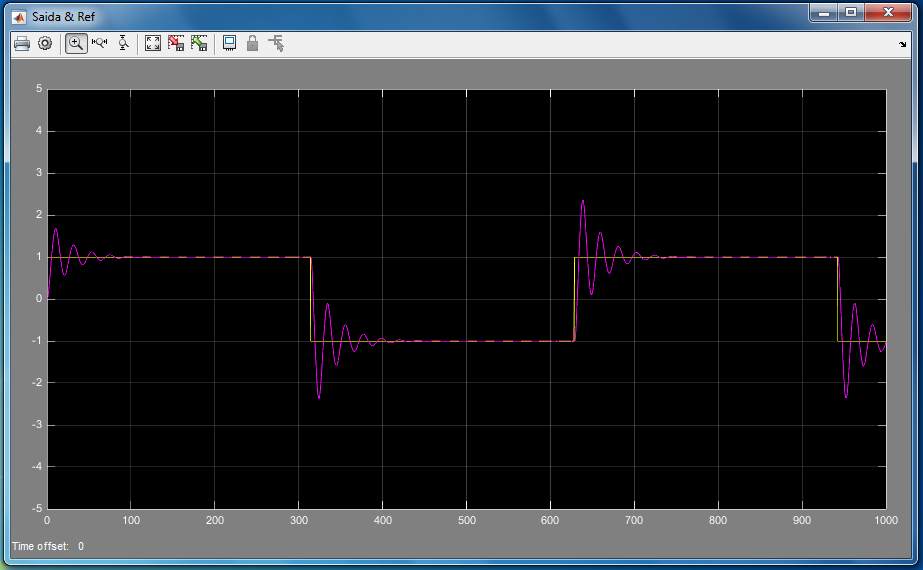
\includegraphics[scale=0.3]{Images/Mamdani_9_square.png}
  \caption{Saída obtida (a roxo) e esperada (a amarelo), utilizando a onda quadrada como referência e um controlador \emph{Mamdani} de $9$ regras}
\end{figure}

\begin{figure}[h]
  \centering
      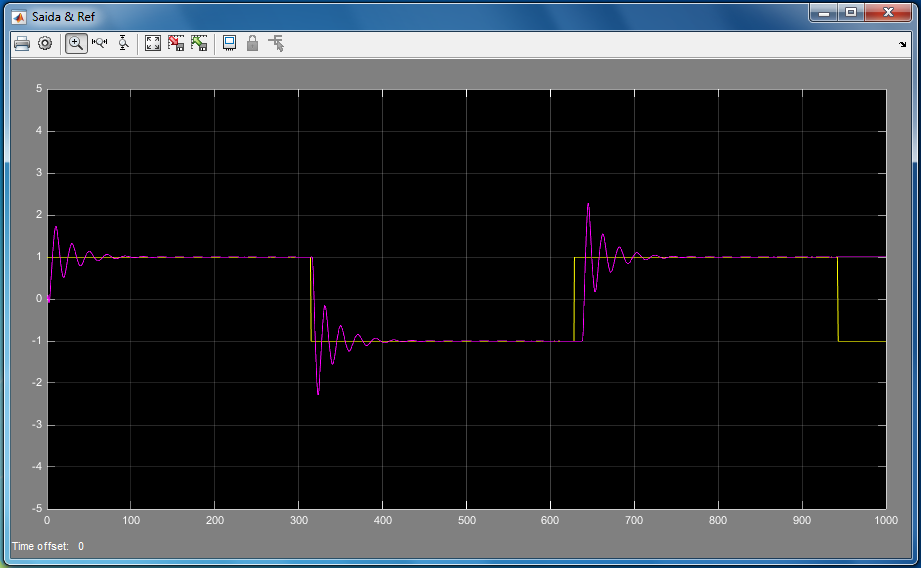
\includegraphics[scale=0.3]{Images/Mamdani_9_square_actuator.png}
  \caption{Saída obtida (a roxo) e esperada (a amarelo), utilizando a onda quadrada como referência e um controlador \emph{Mamdani} de $9$ regras, e com perturbações no atuador}
\end{figure}

\begin{figure}[h]
  \centering
      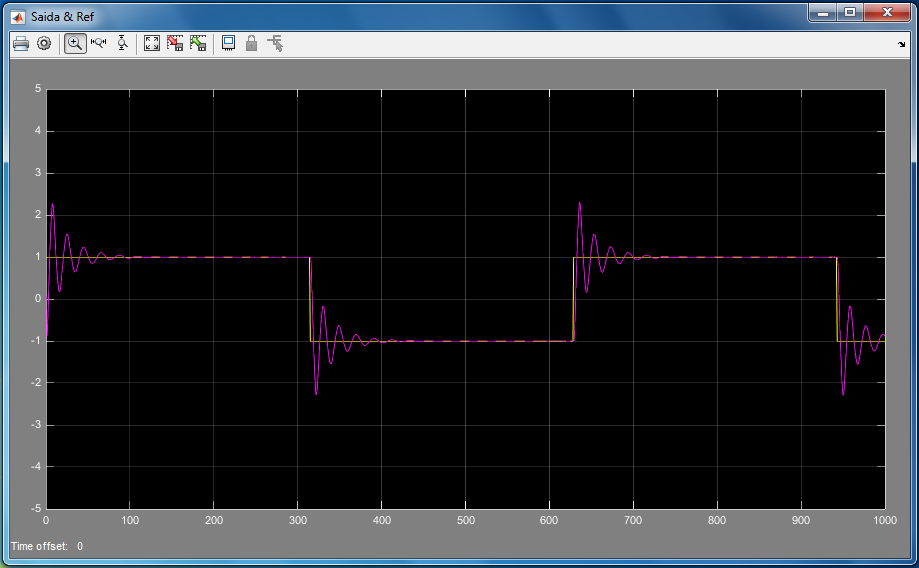
\includegraphics[scale=0.3]{Images/Mamdani_9_square_charge.png}
  \caption{Saída obtida (a roxo) e esperada (a amarelo), utilizando a onda quadrada como referência e um controlador \emph{Mamdani} de $9$ regras, e com perturbações na carga}
\end{figure}


\begin{figure}[h]
  \centering
      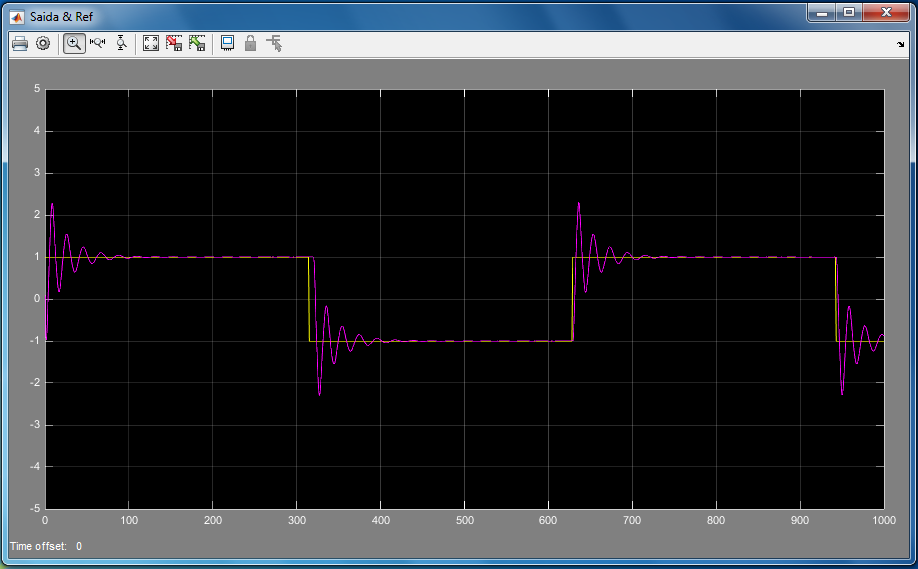
\includegraphics[scale=0.3]{Images/Mamdani_9_square_actuator_charge.png}
  \caption{Saída obtida (a roxo) e esperada (a amarelo), utilizando a onda quadrada como referência e um controlador \emph{Mamdani} de $9$ regras, e com perturbações no atuador e na carga}
\end{figure}

%======================Mamdani_9_sin========================================

\begin{figure}[h]
  \centering
      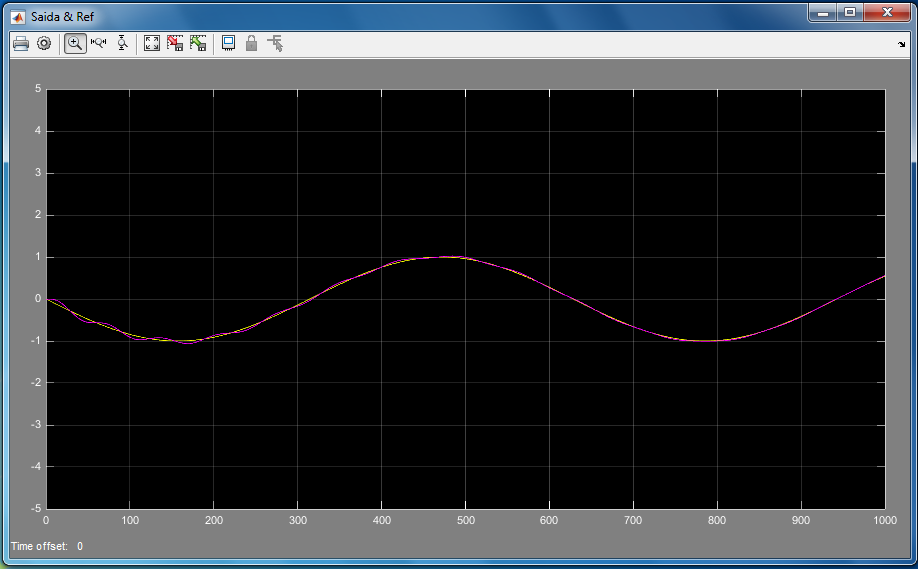
\includegraphics[scale=0.3]{Images/Mamdani_9_sin.png}
  \caption{Saída obtida (a roxo) e esperada (a amarelo), utilizando a onda senoide (seno) como referência e um controlador \emph{Mamdani} de $9$ regras}
\end{figure}

\begin{figure}[h]
  \centering
      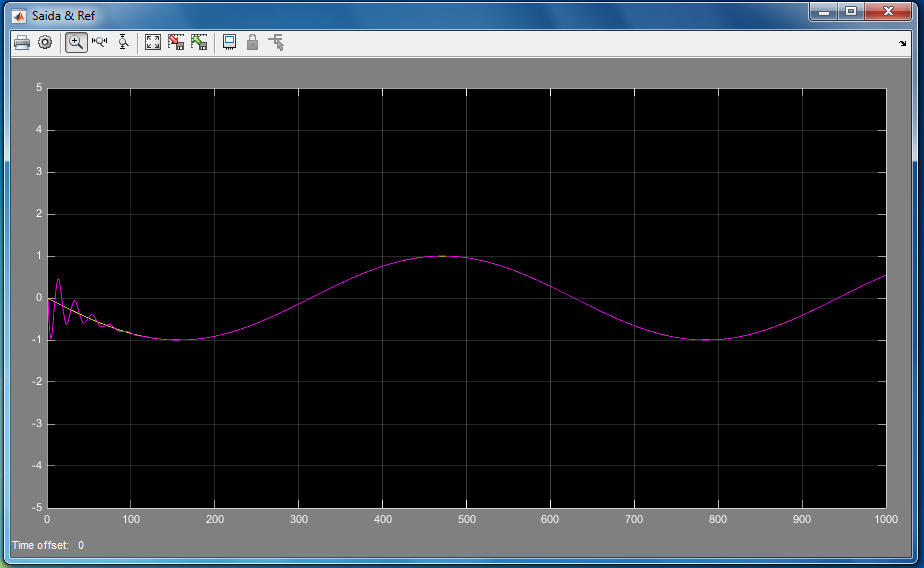
\includegraphics[scale=0.3]{Images/Mamdani_9_sin_actuator.png}
  \caption{Saída obtida (a roxo) e esperada (a amarelo), utilizando a onda senoide (seno) como referência e um controlador \emph{Mamdani} de $9$ regras, e com perturbações no atuador}
\end{figure}

\begin{figure}[h]
  \centering
      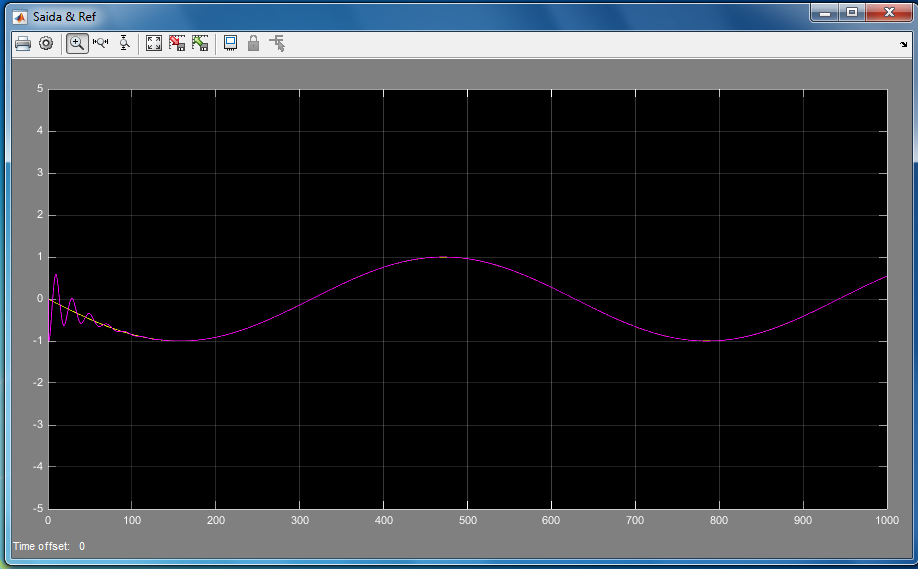
\includegraphics[scale=0.3]{Images/Mamdani_9_sin_charge.png}
  \caption{Saída obtida (a roxo) e esperada (a amarelo), utilizando a onda senoide (seno) como referência e um controlador \emph{Mamdani} de $9$ regras, e com perturbações na carga}
\end{figure}

\begin{figure}[h]
  \centering
      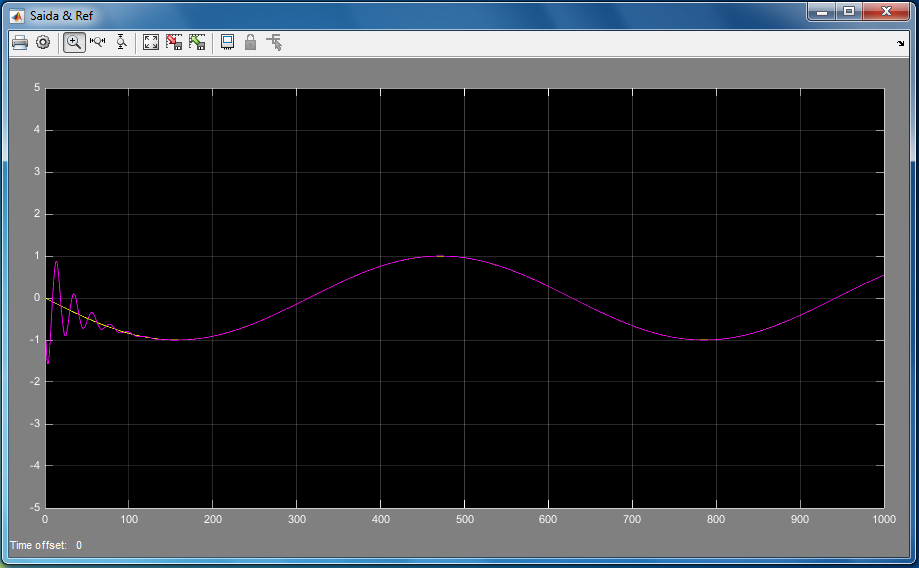
\includegraphics[scale=0.3]{Images/Mamdani_9_sin_actuator_charge.png}
  \caption{Saída obtida (a roxo) e esperada (a amarelo), utilizando a onda senoide (seno) como referência e um controlador \emph{Mamdani} de $9$ regras, e com perturbações no atuador e na carga}
\end{figure}

%======================Mamdani_25_square====================================

\begin{figure}[h]
  \centering
      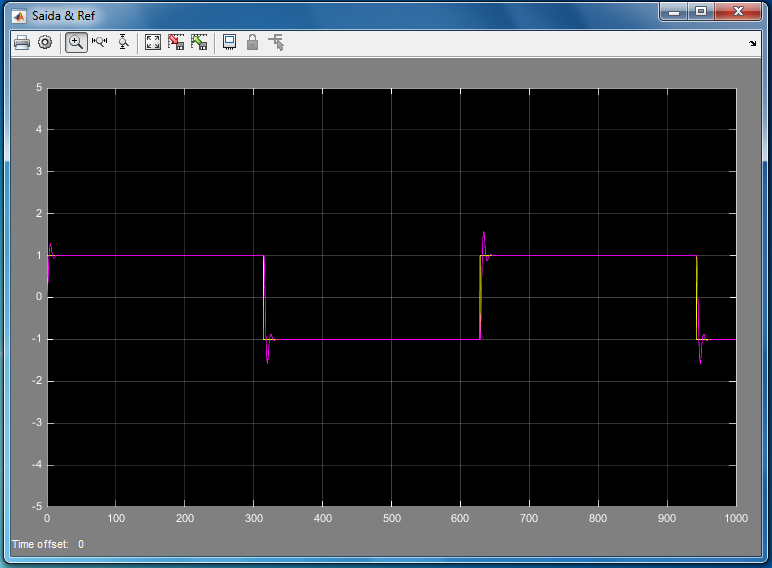
\includegraphics[scale=0.3]{Images/Mamdani_25_square.png}
  \caption{Saída obtida (a roxo) e esperada (a amarelo), utilizando a onda quadrada como referência e um controlador \emph{Mamdani} de $25$ regras}
\end{figure}

\begin{figure}[h]
  \centering
      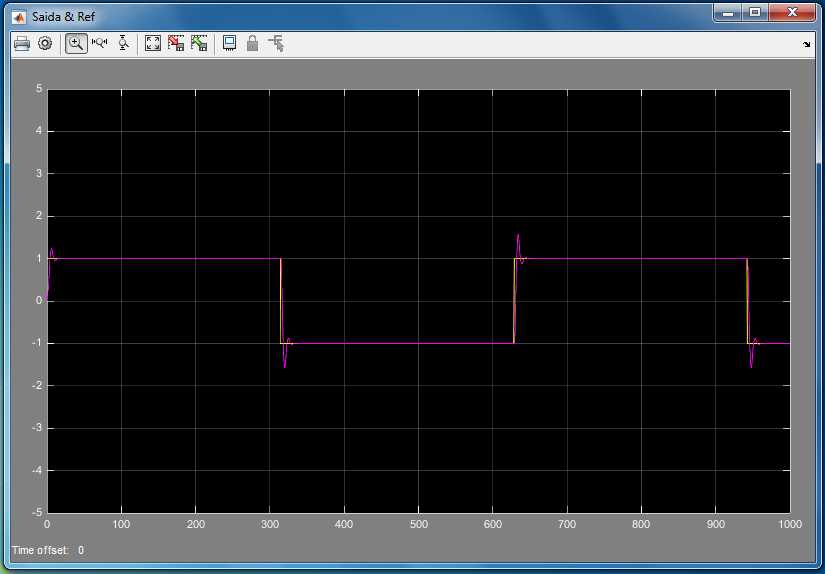
\includegraphics[scale=0.3]{Images/Mamdani_25_square_actuator.png}
  \caption{Saída obtida (a roxo) e esperada (a amarelo), utilizando a onda quadrada como referência e um controlador \emph{Mamdani} de $25$ regras, e com perturbações no atuador}
\end{figure}

\begin{figure}[h]
  \centering
      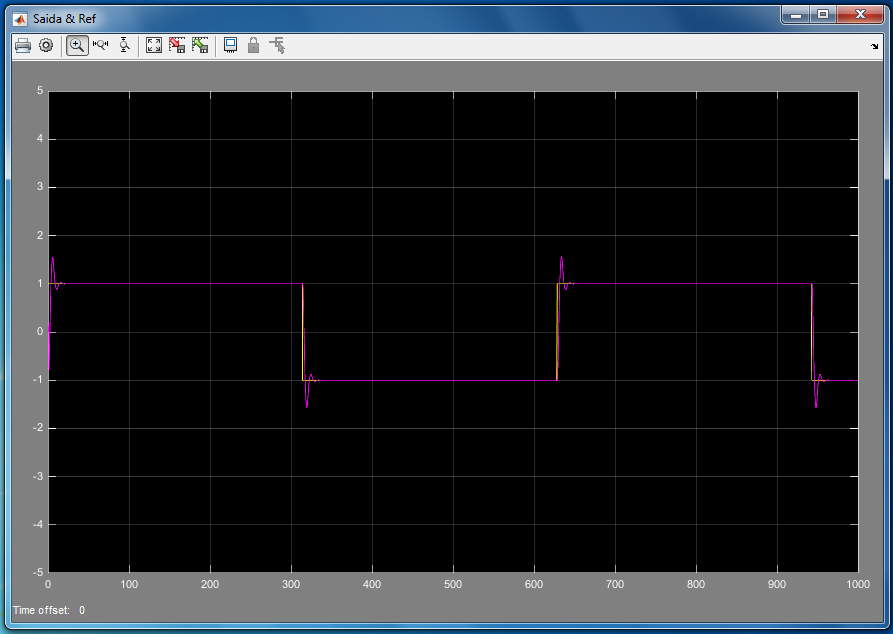
\includegraphics[scale=0.3]{Images/Mamdani_25_square_charge.png}
  \caption{Saída obtida (a roxo) e esperada (a amarelo), utilizando a onda quadrada como referência e um controlador \emph{Mamdani} de $25$ regras, e com perturbações na carga}
\end{figure}

\begin{figure}[h]
  \centering
      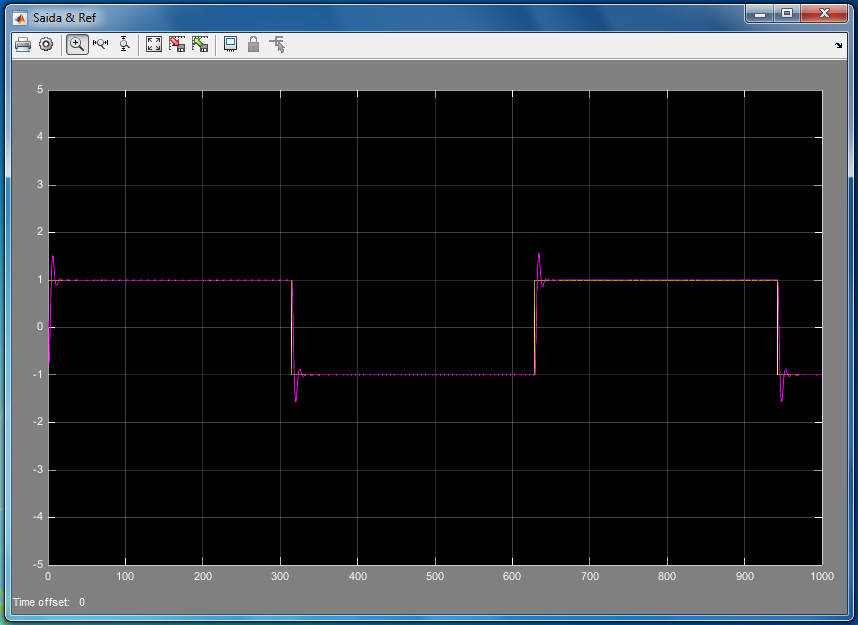
\includegraphics[scale=0.3]{Images/Mamdani_25_square_actuator_charge.png}
  \caption{Saída obtida (a roxo) e esperada (a amarelo), utilizando a onda quadrada como referência e um controlador \emph{Mamdani} de $25$ regras, e com perturbações no atuador e na carga}
\end{figure}

%======================Mamdani_25_sin=======================================

\begin{figure}[h]
  \centering
      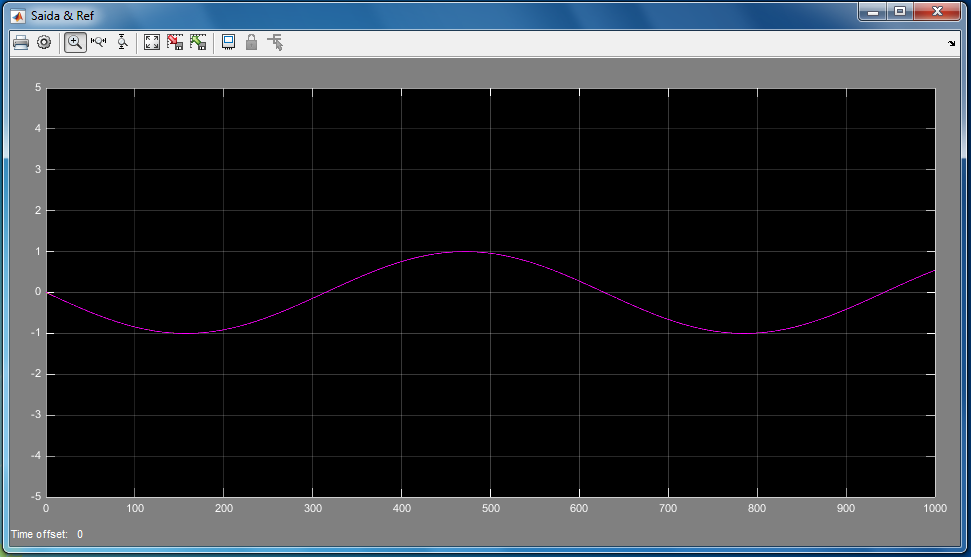
\includegraphics[scale=0.3]{Images/Mamdani_25_sin.png}
  \caption{Saída obtida (a roxo) e esperada (a amarelo), utilizando a onda senoide (seno) como referência e um controlador \emph{Mamdani} de $25$ regras}
\end{figure}

\begin{figure}[h]
  \centering
      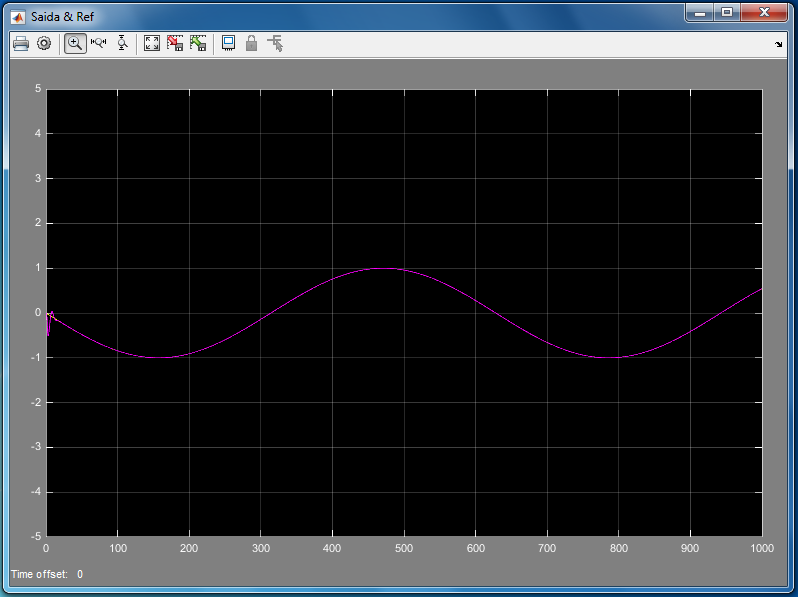
\includegraphics[scale=0.3]{Images/Mamdani_25_sin_actuator.png}
  \caption{Saída obtida (a roxo) e esperada (a amarelo), utilizando a onda senoide (seno) como referência e um controlador \emph{Mamdani} de $25$ regras, e com perturbações no atuador}
\end{figure}

\begin{figure}[h]
  \centering
      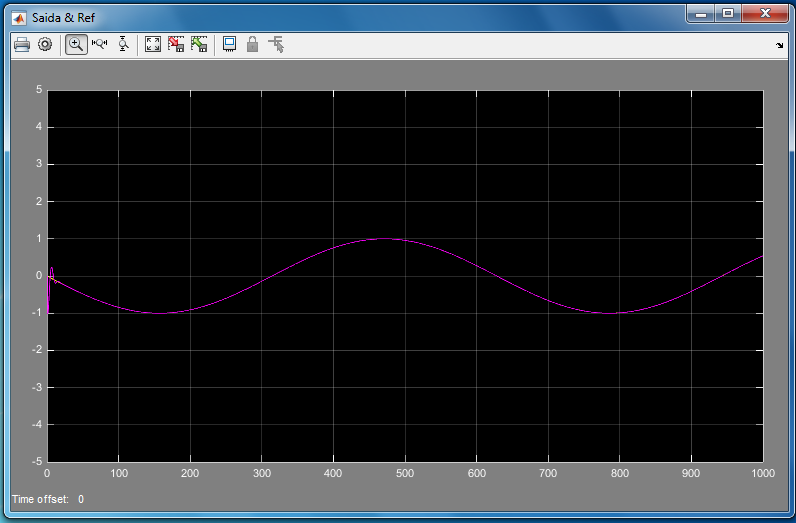
\includegraphics[scale=0.3]{Images/Mamdani_25_sin_charge.png}
  \caption{Saída obtida (a roxo) e esperada (a amarelo), utilizando a onda senoide (seno) como referência e um controlador \emph{Mamdani} de $25$ regras, e com perturbações na carga}
\end{figure}

\begin{figure}[h]
  \centering
      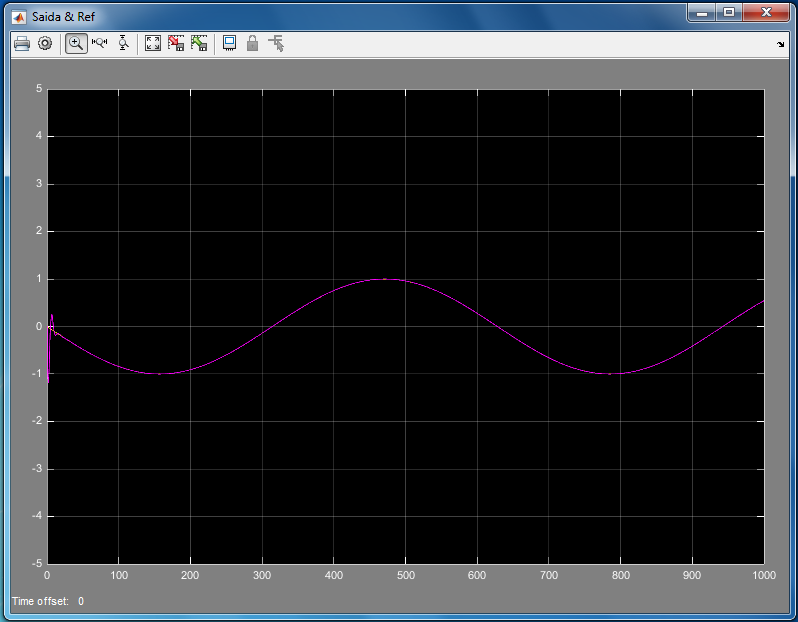
\includegraphics[scale=0.3]{Images/Mamdani_25_sin_actuator_charge.png}
  \caption{Saída obtida (a roxo) e esperada (a amarelo), utilizando a onda senoide (seno) como referência e um controlador \emph{Mamdani} de $25$ regras, e com perturbações no atuador e na carga}
\end{figure}

%======================Sugeno_9_square======================================

\begin{figure}[h]
  \centering
      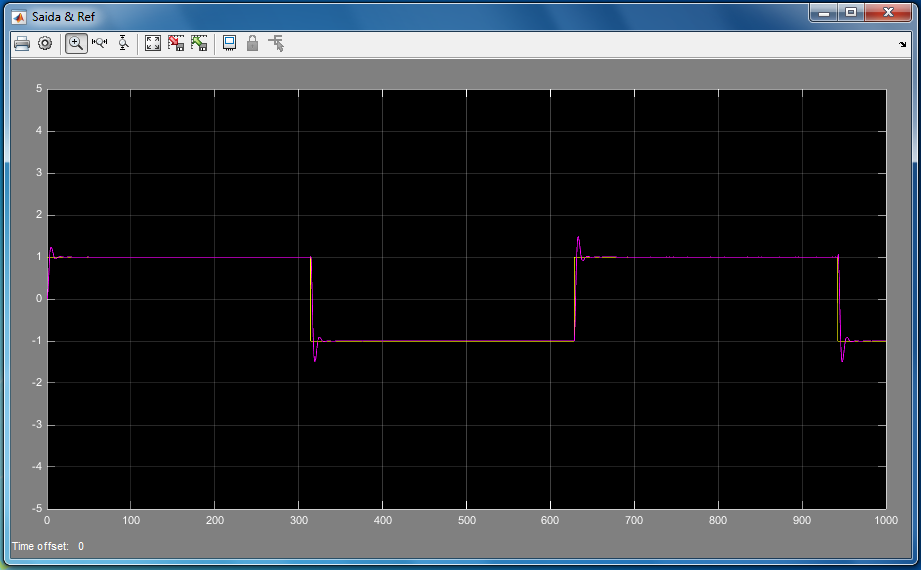
\includegraphics[scale=0.3]{Images/Sugeno_9_square.png}
  \caption{Saída obtida (a roxo) e esperada (a amarelo), utilizando a onda quadrada como referência e um controlador \emph{Sugeno} de $9$ regras}
\end{figure}

\begin{figure}[h]
  \centering
      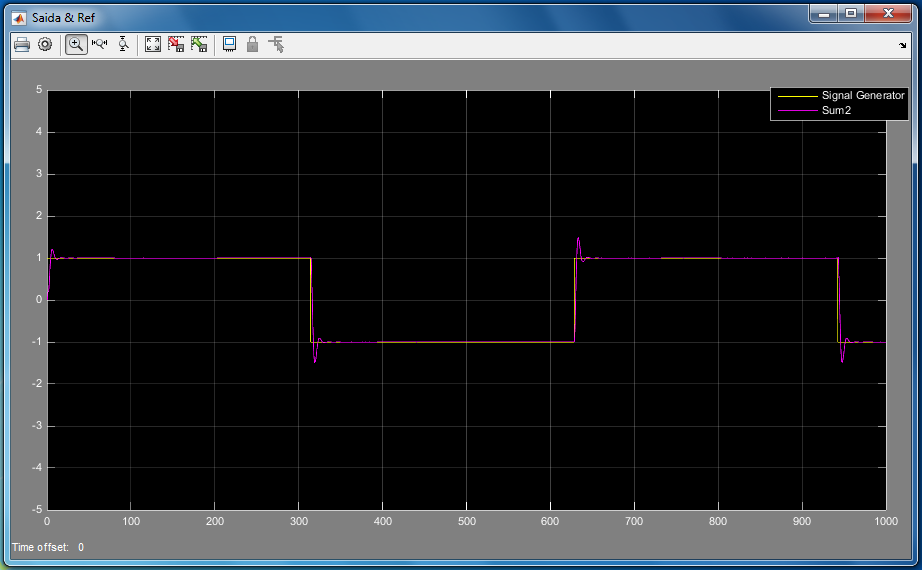
\includegraphics[scale=0.3]{Images/Sugeno_9_square_actuator.png}
  \caption{Saída obtida (a roxo) e esperada (a amarelo), utilizando a onda quadrada como referência e um controlador \emph{Sugeno} de $9$ regras, e com perturbações no atuador}
\end{figure}

\clearpage

\begin{figure}[h]
  \centering
      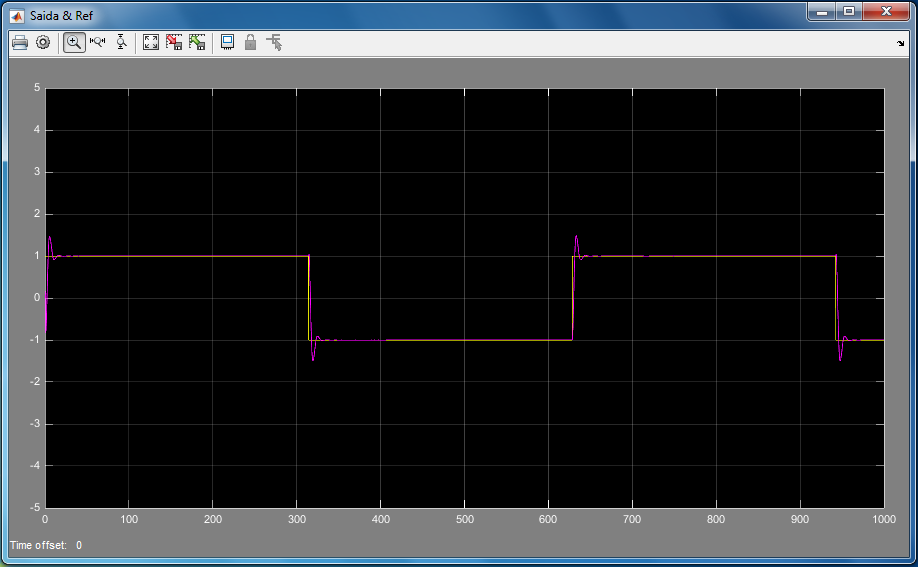
\includegraphics[scale=0.3]{Images/Sugeno_9_square_charge.png}
  \caption{Saída obtida (a roxo) e esperada (a amarelo), utilizando a onda quadrada como referência e um controlador \emph{Sugeno} de $9$ regras, e com perturbações na carga}
\end{figure}

\begin{figure}[h]
  \centering
      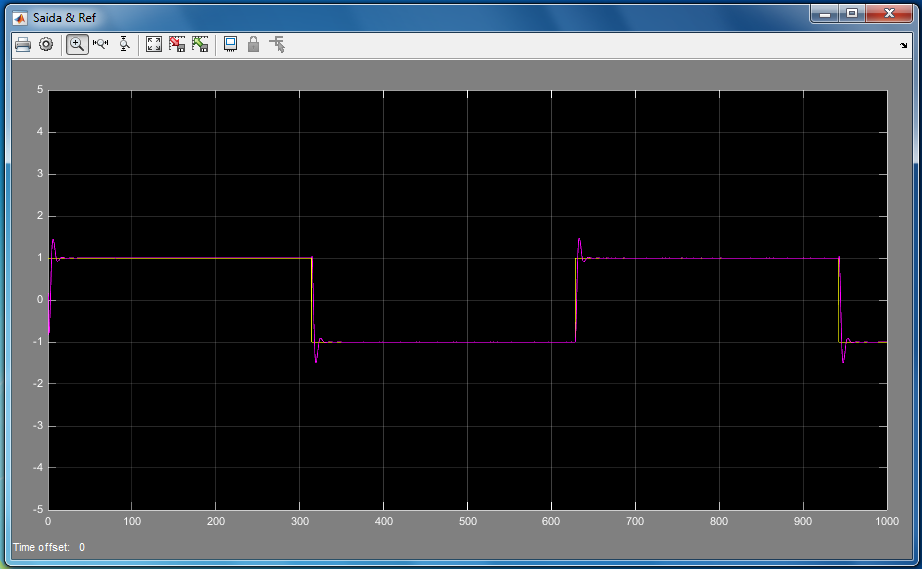
\includegraphics[scale=0.3]{Images/Sugeno_9_square_actuator_charge.png}
  \caption{Saída obtida (a roxo) e esperada (a amarelo), utilizando a onda quadrada como referência e um controlador \emph{Sugeno} de $9$ regras, e com perturbações no atuador e na carga}
\end{figure}

%======================Sugeno_9_sin=========================================

\begin{figure}[h]
  \centering
      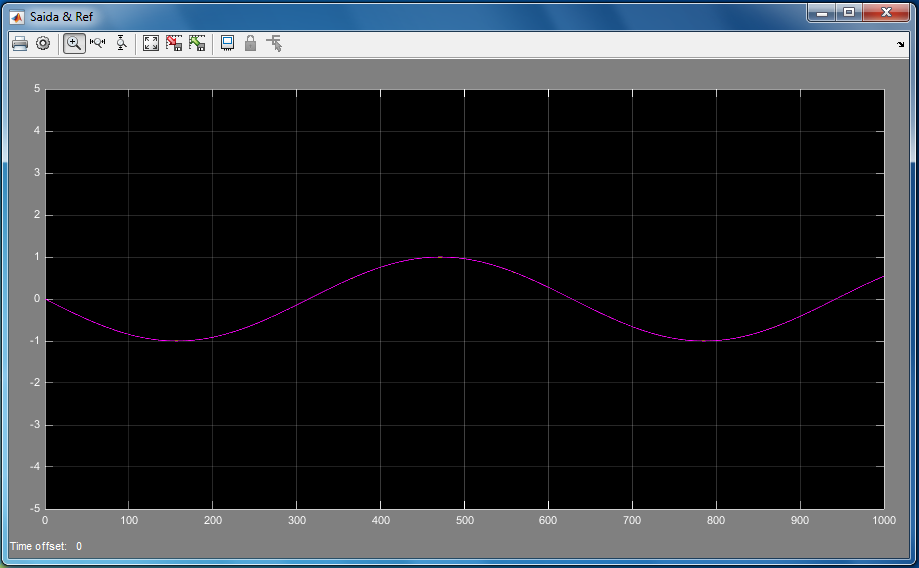
\includegraphics[scale=0.3]{Images/Sugeno_9_sin.png}
  \caption{Saída obtida (a roxo) e esperada (a amarelo), utilizando a onda senoide (seno) como referência e um controlador \emph{Sugeno} de $9$ regras}
\end{figure}

\begin{figure}[h]
  \centering
      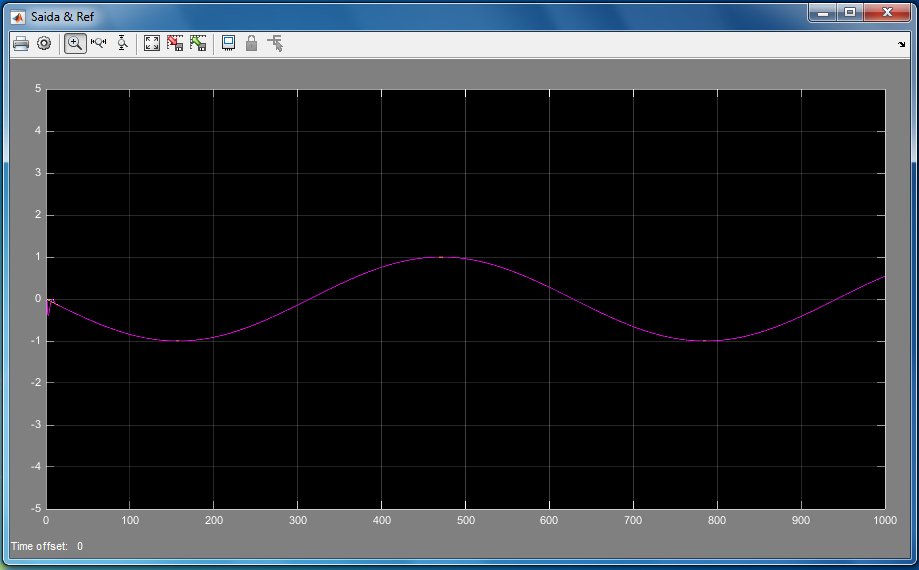
\includegraphics[scale=0.3]{Images/Sugeno_9_sin_actuator.png}
  \caption{Saída obtida (a roxo) e esperada (a amarelo), utilizando a onda senoide (seno) como referência e um controlador \emph{Sugeno} de $9$ regras, e com perturbações no atuador}
\end{figure}

\begin{figure}[h]
  \centering
      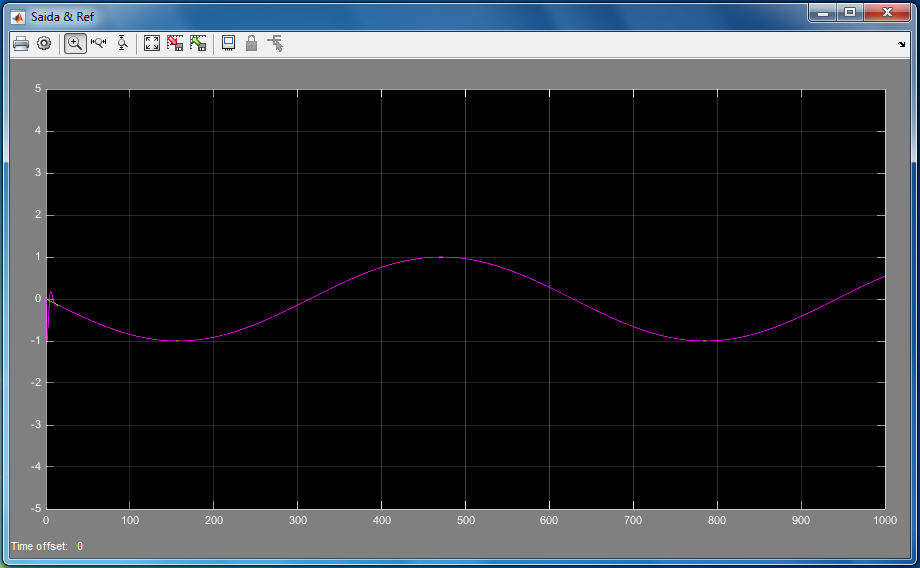
\includegraphics[scale=0.3]{Images/Sugeno_9_sin_charge.png}
  \caption{Saída obtida (a roxo) e esperada (a amarelo), utilizando a onda senoide (seno) como referência e um controlador \emph{Sugeno} de $9$ regras, e com perturbações na carga}
\end{figure}

\begin{figure}[h]
  \centering
      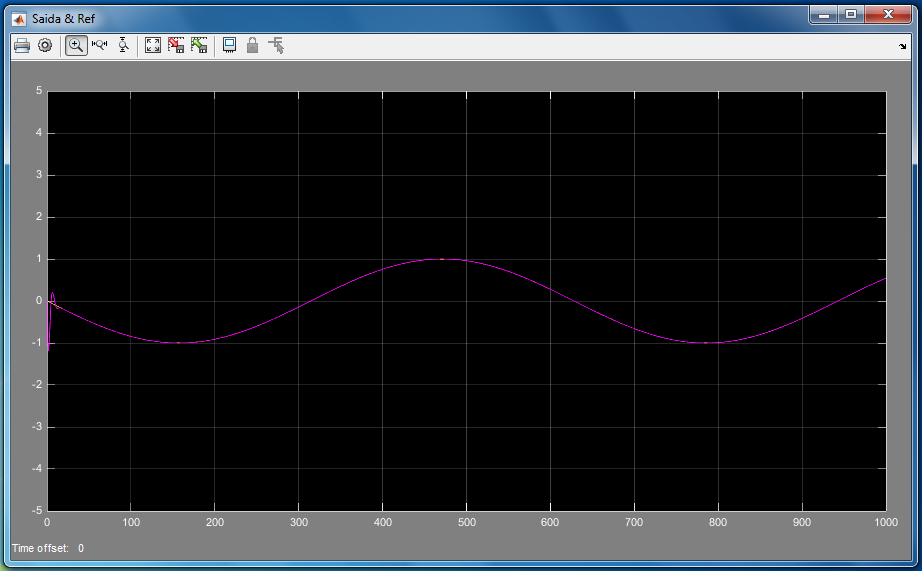
\includegraphics[scale=0.3]{Images/Sugeno_9_sin_actuator_charge.png}
  \caption{Saída obtida (a roxo) e esperada (a amarelo), utilizando a onda senoide (seno) como referência e um controlador \emph{Sugeno} de $9$ regras, e com perturbações no atuador e na carga}
\end{figure}

%======================Sugeno_25_square=====================================

\begin{figure}[h]
  \centering
      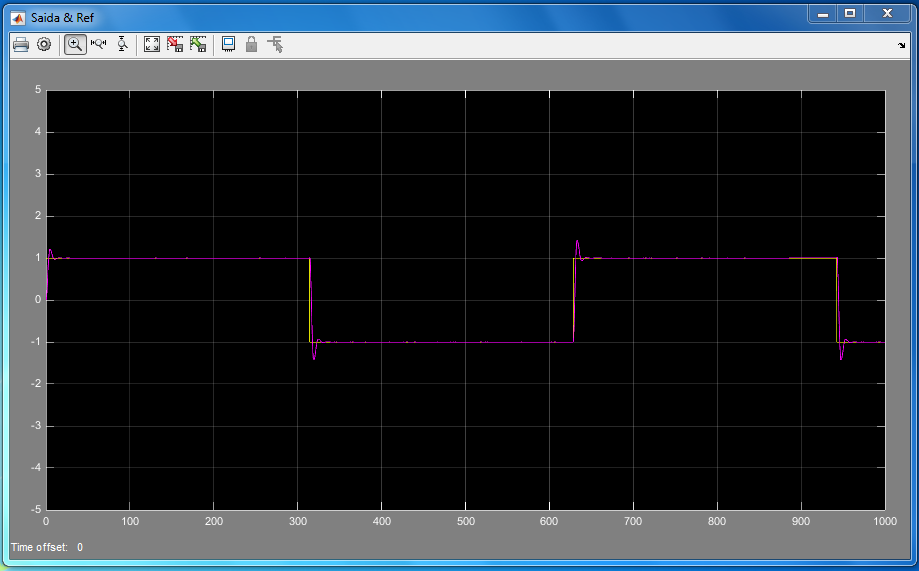
\includegraphics[scale=0.3]{Images/Sugeno_25_square.png}
  \caption{Saída obtida (a roxo) e esperada (a amarelo), utilizando a onda quadrada como referência e um controlador \emph{Sugeno} de $25$ regras}
\end{figure}

\begin{figure}[h]
  \centering
      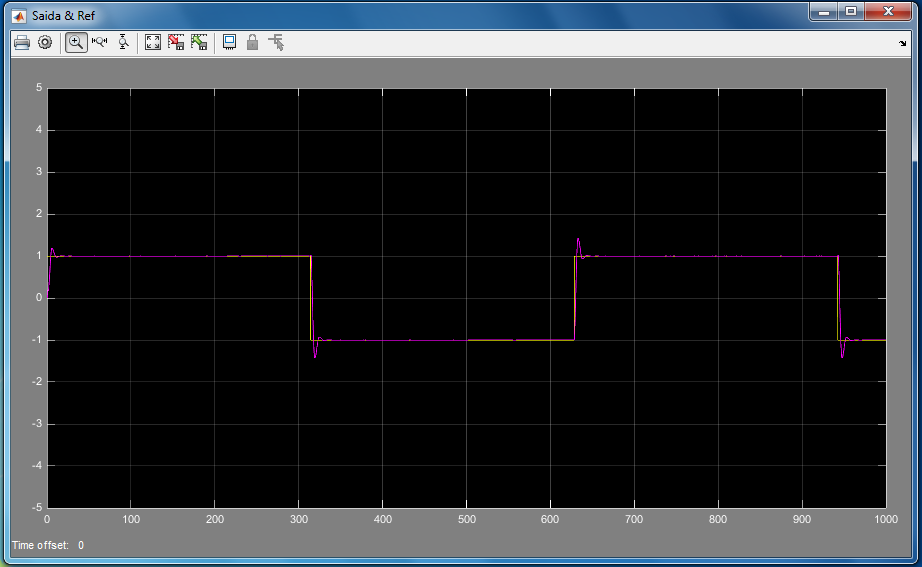
\includegraphics[scale=0.3]{Images/Sugeno_25_square_actuator.png}
  \caption{Saída obtida (a roxo) e esperada (a amarelo), utilizando a onda quadrada como referência e um controlador \emph{Sugeno} de $25$ regras, e com perturbações no atuador}
\end{figure}

\begin{figure}[h]
  \centering
      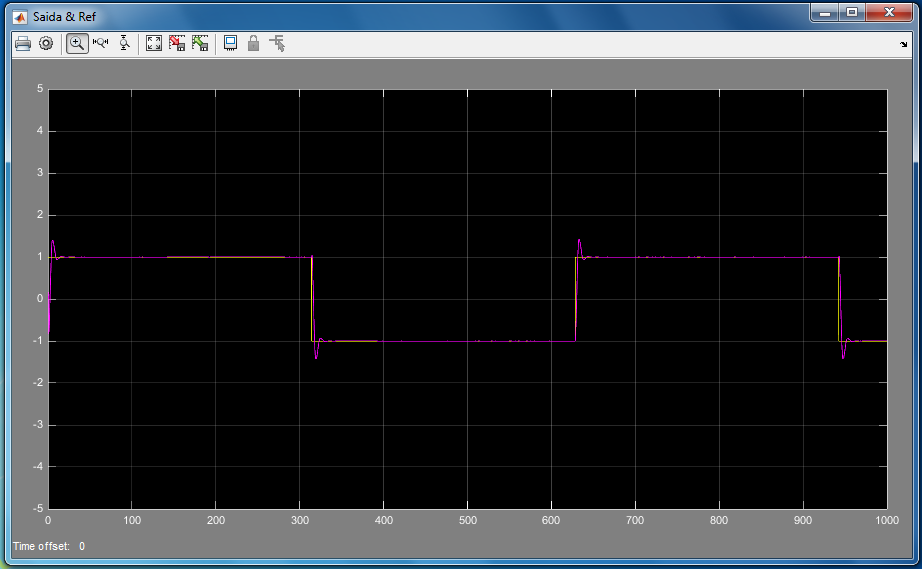
\includegraphics[scale=0.3]{Images/Sugeno_25_square_charge.png}
  \caption{Saída obtida (a roxo) e esperada (a amarelo), utilizando a onda quadrada como referência e um controlador \emph{Sugeno} de $9$ regras, e com perturbações na carga}
\end{figure}

\begin{figure}[h]
  \centering
      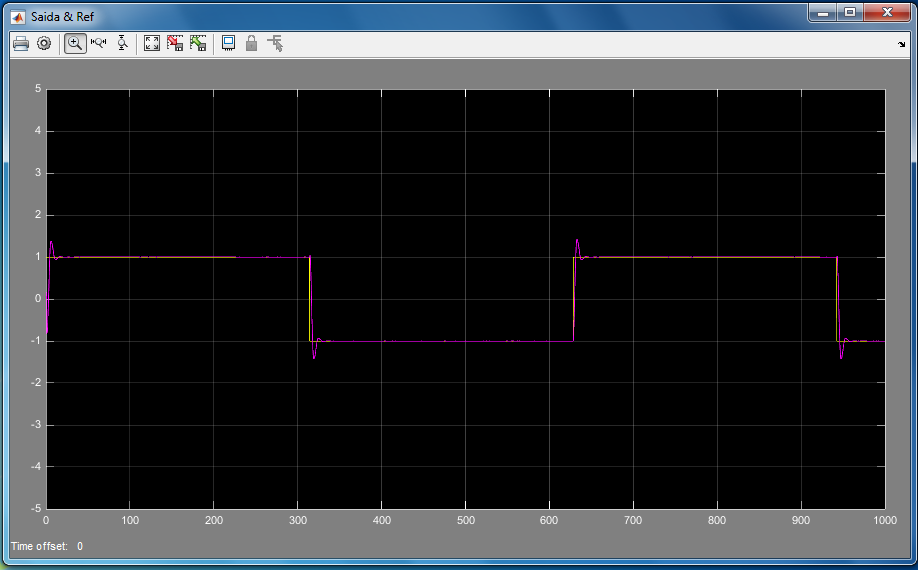
\includegraphics[scale=0.3]{Images/Sugeno_25_square_actuator_charge.png}
  \caption{Saída obtida (a roxo) e esperada (a amarelo), utilizando a onda quadrada como referência e um controlador \emph{Sugeno} de $25$ regras, e com perturbações no atuador e na carga}
\end{figure}

%======================Sugeno_25_sin========================================

\begin{figure}[h]
  \centering
      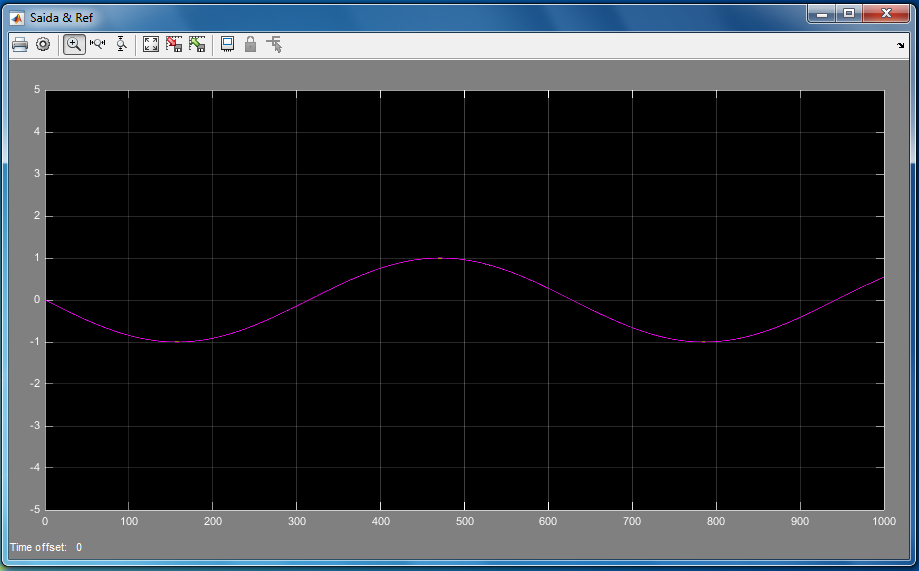
\includegraphics[scale=0.3]{Images/Sugeno_25_sin.png}
  \caption{Saída obtida (a roxo) e esperada (a amarelo), utilizando a onda senoide (seno) como referência e um controlador \emph{Sugeno} de $25$ regras}
\end{figure}

\begin{figure}[h]
  \centering
      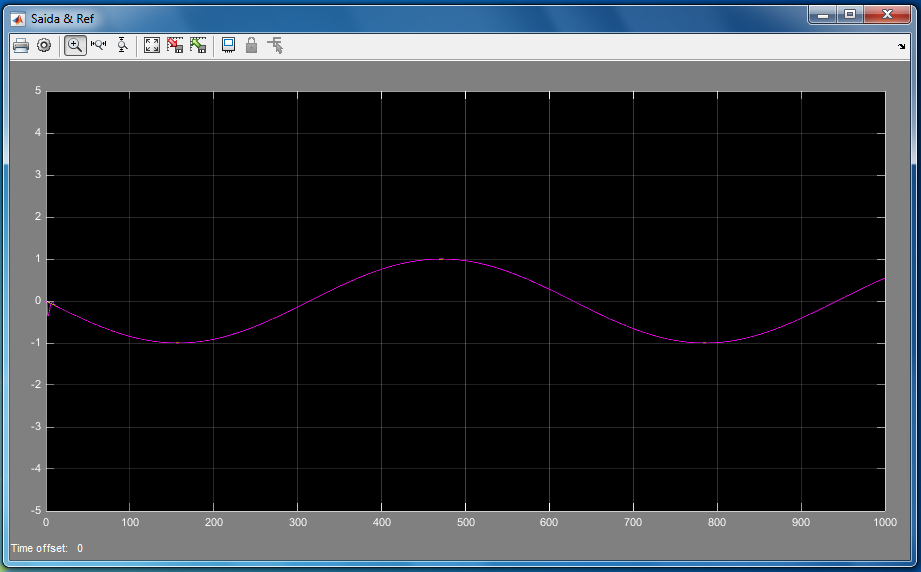
\includegraphics[scale=0.3]{Images/Sugeno_25_sin_actuator.png}
  \caption{Saída obtida (a roxo) e esperada (a amarelo), utilizando a onda senoide (seno) como referência e um controlador \emph{Sugeno} de $25$ regras, e com perturbações no atuador}
\end{figure}

\begin{figure}[h]
  \centering
      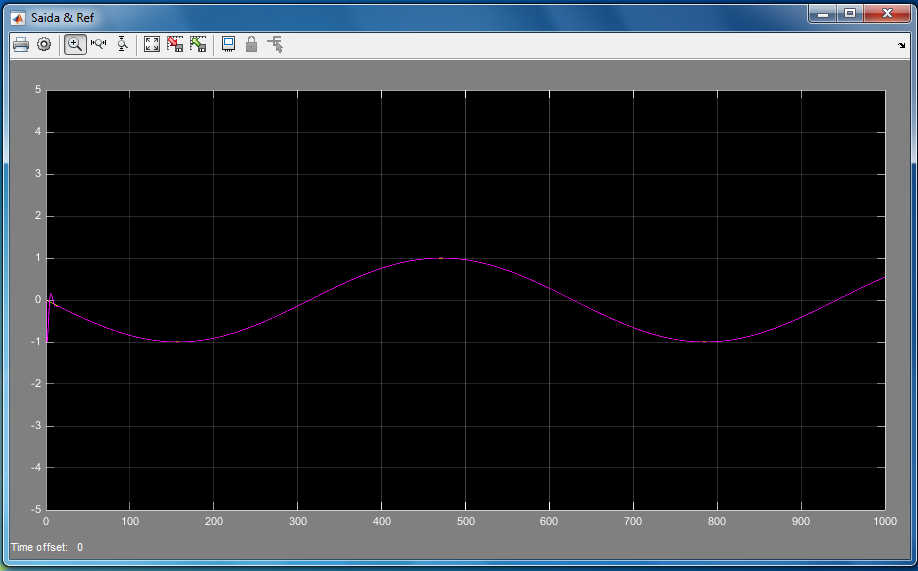
\includegraphics[scale=0.3]{Images/Sugeno_25_sin_charge.png}
  \caption{Saída obtida (a roxo) e esperada (a amarelo), utilizando a onda senoide (seno) como referência e um controlador \emph{Sugeno} de $25$ regras, e com perturbações na carga}
\end{figure}

\begin{figure}[h]
  \centering
      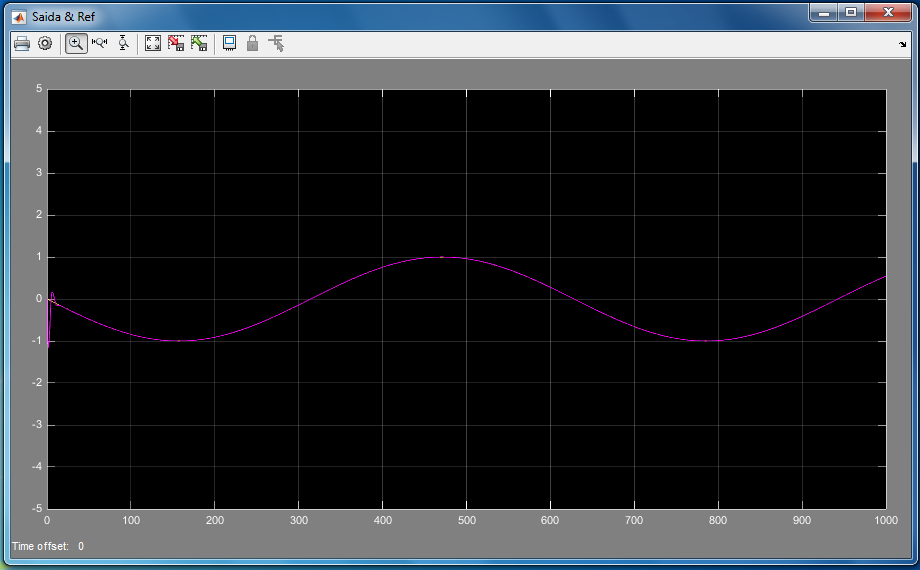
\includegraphics[scale=0.3]{Images/Sugeno_25_sin_actuator_charge.png}
  \caption{Saída obtida (a roxo) e esperada (a amarelo), utilizando a onda senoide (seno) como referência e um controlador \emph{Sugeno} de $25$ regras, e com perturbações no atuador e na carga}
\end{figure}

\end{document}